\section{Experimentación}
\subsection{Búsqueda de la mejor solucion}

\subsubsection{Ejercicio 1}
Para el ejercicio 1, implementamos un algoritmo simple para probar distintas ejecuciones y quedarnos con las soluciones que convergian. 

La idea general del algoritmo es iterar variando el modo de ejecucion (Sanger y Oja) y variando el \textbf{Learning Rate}. Por otro lado tambien modificamos a mano el parametro de epsilon para poder comparar y hacer la experimentacion. Es decir, para cada epsilon encontramos las mejores soluciones.

En el caso de \textbf{Sanger} se ejecuta variando el \textbf{Learning Rate} pero en caso de que una solucion converga, se corta, dado que una vez que se encuentra una solucion en Sanger esta es \textbf{la} solucion.

En el caso de \textbf{Oja} se ejecuta variando el \textbf{Learning Rate} y en caso de que converga guardamos la solucion y en caso de que no, no la guardamos.

El algoritmo para hacer estas pruebas es el siguiente:


\begin{lstlisting}[caption=pruebas]
	
	def pruebas(dataset,save_file,max_epochs=5000):
	best_params_oja = []
	best_params_sanger = -1
	for m in [0, 1]:
		for lrate in np.linspace(0.001, 0.1, 20):
			convergio = train_Ej1(dataset, save_file, 3, lrate, max_epochs,m)
			if convergio and not m:
				best_params_sanger = lrate
				break
			if convergio and m:
				best_params_oja.append(lrate)
	return best_params_sanger, best_params_oja

\end{lstlisting}

\subsubsection{Ejercicio 2}

\subsection{Ejercicio 1}

Como se explico anteriormente se corrio nuestro algoritmo de pruebas para encotnrar las mejores soluciones en cada modo. El algoritmo de pruebas es corrio con distintos \textbf{epsilons} y obtuvimos lo siguientes resultados:

\begin{tabular}{|l|l|l|}
\hline
Epsilon & Sanger & Oja \\ \hline
0.01           & -1      	& [0.001]  \\ \hline
0.015          & 0.001      & [0.001]   \\ \hline
0.02           & 0.001      & [0.001]   \\ \hline
0.05           & 0.001      & [0.001, 0.0062105263157894736, 0.011421052631578946]   \\ \hline
0.1            & 0.001      & [0.001, 0.006211, 0.0114211, 0.01664, 0.021843]   \\ \hline

\end{tabular}


En la tabla se puede ver para cada epsilon, los resultados obtenidos con cada algoritmo. En caso de Sanger si tiene un \textbf{-1} es porque no convergio a una solucion, en cambio, si converge se muestra el valor del Learning Rate. En el caso de Oja, el valor de la celda en la tabla es una lista con los Learning Rates que convergieron a una solucion.

En todos los casos se analizaron los graficos para ver que solucion es mejor que otra y pudimos ver que:

Con un epsilon de 0.1 en sanger obtuvimos un grafico como el siguiente:


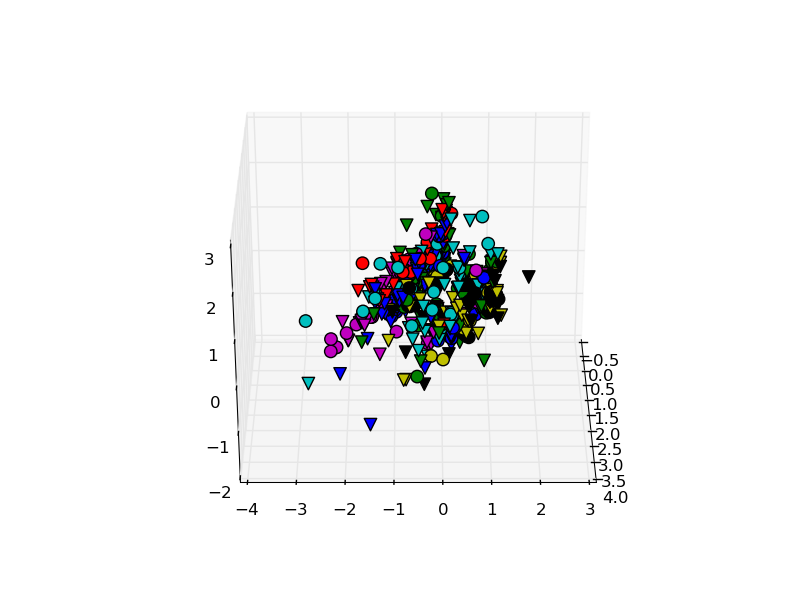
\includegraphics[width=0.5\textwidth]{img/ej1_sanger_01_20}
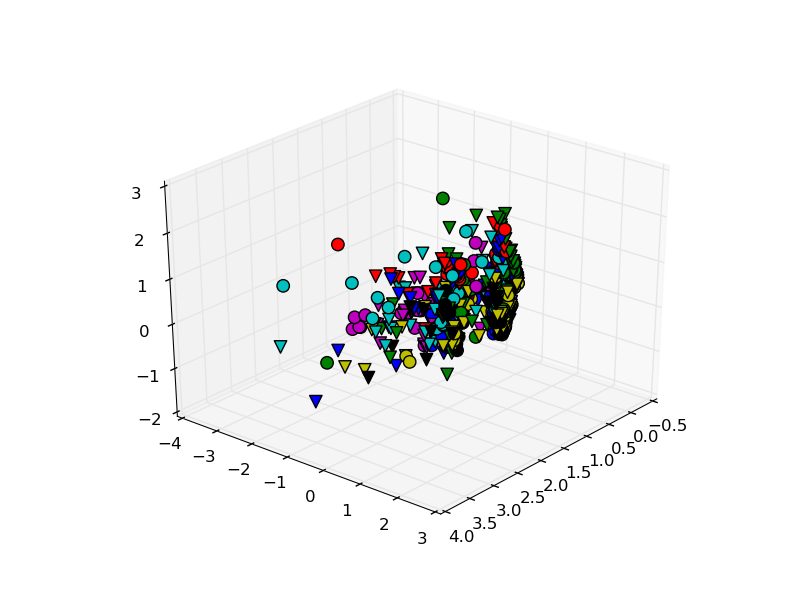
\includegraphics[width=0.5\textwidth]{img/ej1_sanger_01_40}
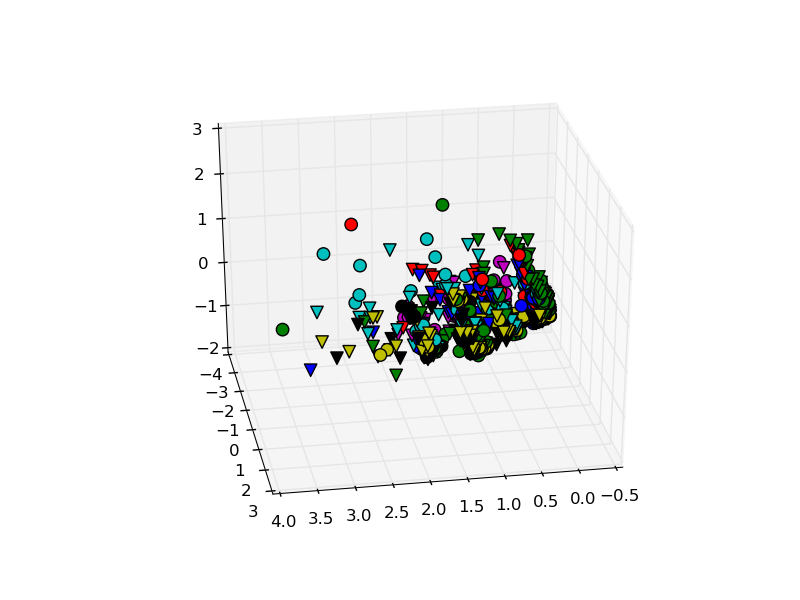
\includegraphics[width=0.5\textwidth]{img/ej1_sanger_01_80}
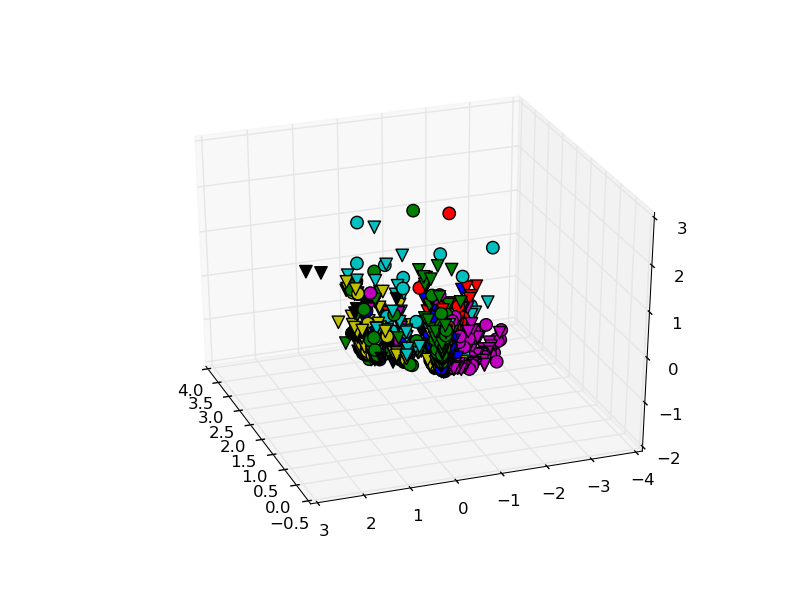
\includegraphics[width=0.5\textwidth]{img/ej1_sanger_01_160}
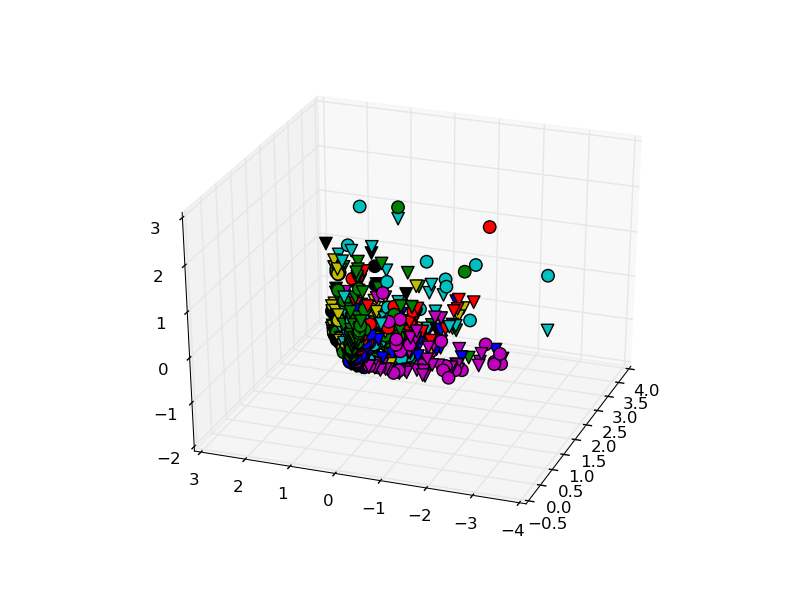
\includegraphics[width=0.5\textwidth]{img/ej1_sanger_01_200}
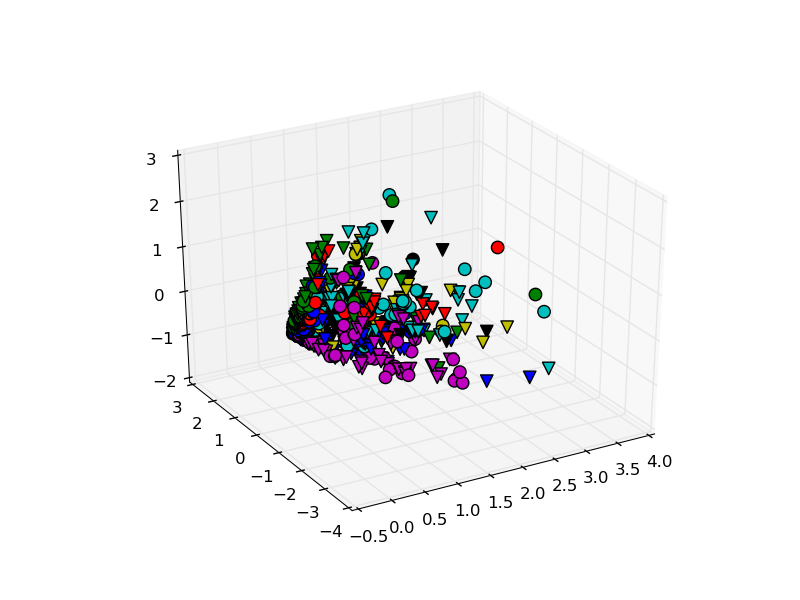
\includegraphics[width=0.5\textwidth]{img/ej1_sanger_01_240}


En este grafico lo que notamos muchos puntos estan dispersos, pero no solo dispersos, sino que son puntos dispersos de \textbf{distintos categorias}. 

Es dificil apreciar una agrupacion particular de un culor especifico, es decir, todos los colores estan un poco mezclados.

En particular el color amarillo se mezcla mucho con el verde, y el color rojo esta desparramado. 

Se nota tambien que el color violeta, al igual que el verde estan cerca de agruparse.

En algunos puntos se nota una mezcla intensa de color amarrilo y verde. Mientras que en otros lugares se nota esta mezcla pero de violeta, verde y azul.

Una particularidad de este grafico, es que el color rojo no resalta tanto y tiene un valor atipico.

con el mismo epsilon y con un learning rate de 0.001, en Oja obtuvimos 

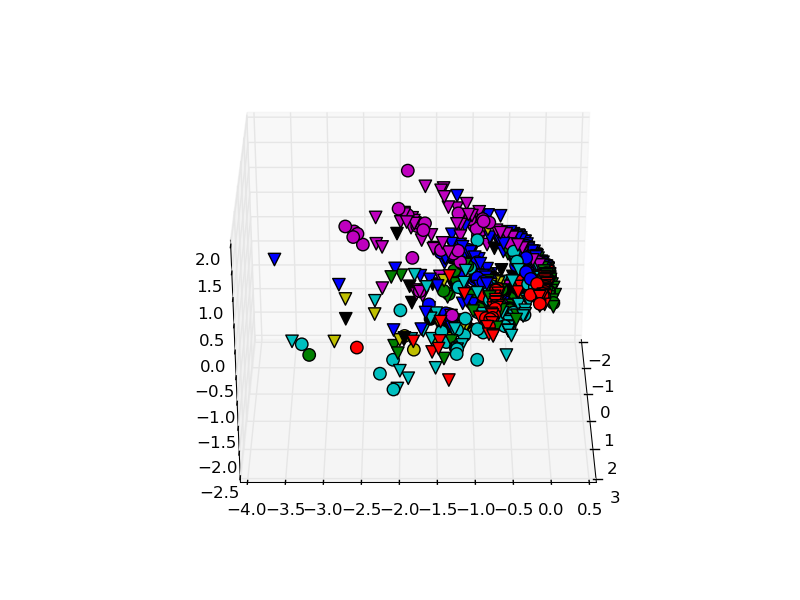
\includegraphics[width=0.5\textwidth]{img/ej1_oja_01_20}
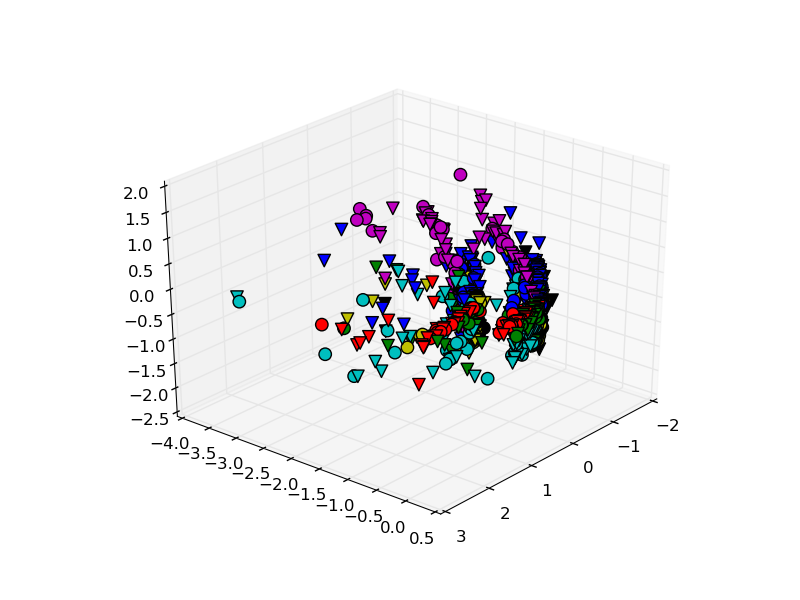
\includegraphics[width=0.5\textwidth]{img/ej1_oja_01_40}
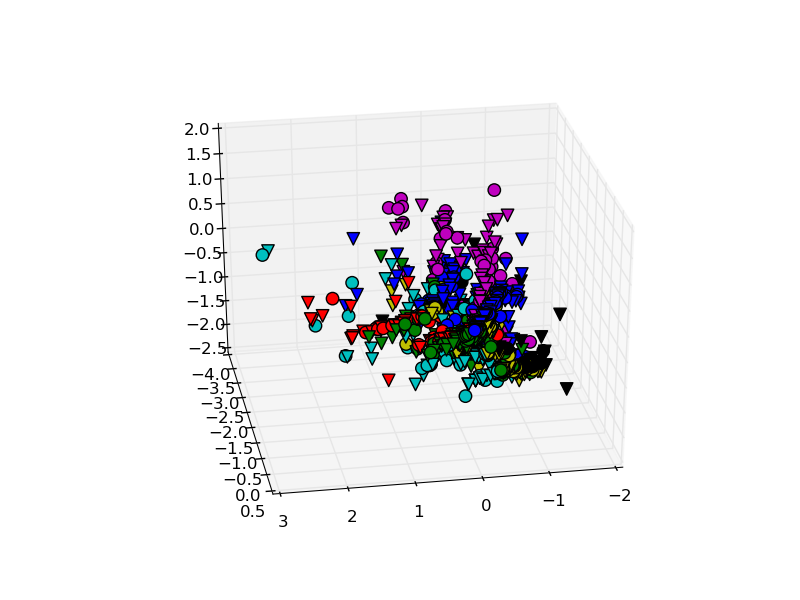
\includegraphics[width=0.5\textwidth]{img/ej1_oja_01_80}
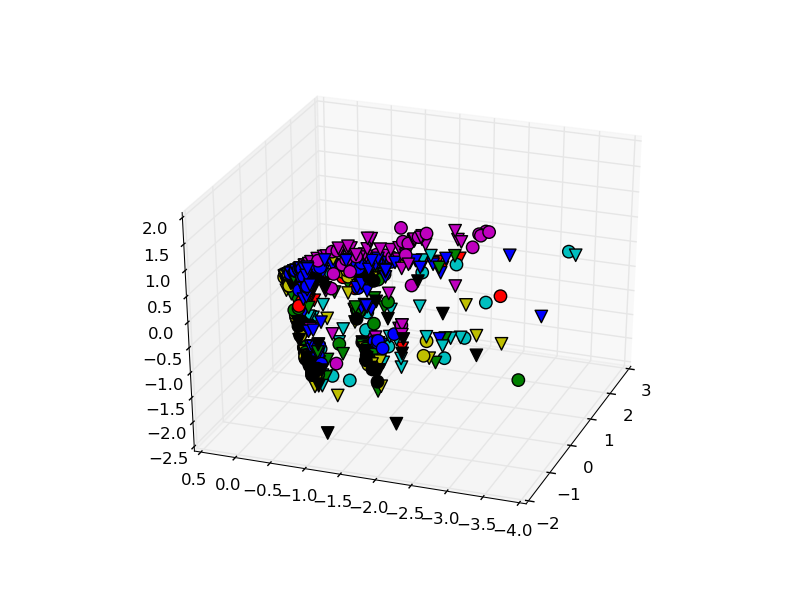
\includegraphics[width=0.5\textwidth]{img/ej1_oja_01_200}
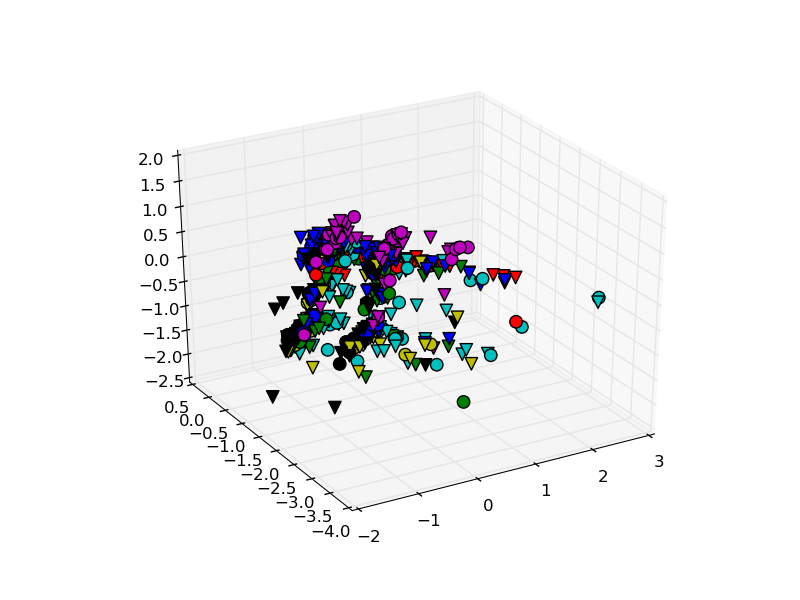
\includegraphics[width=0.5\textwidth]{img/ej1_oja_01_240}
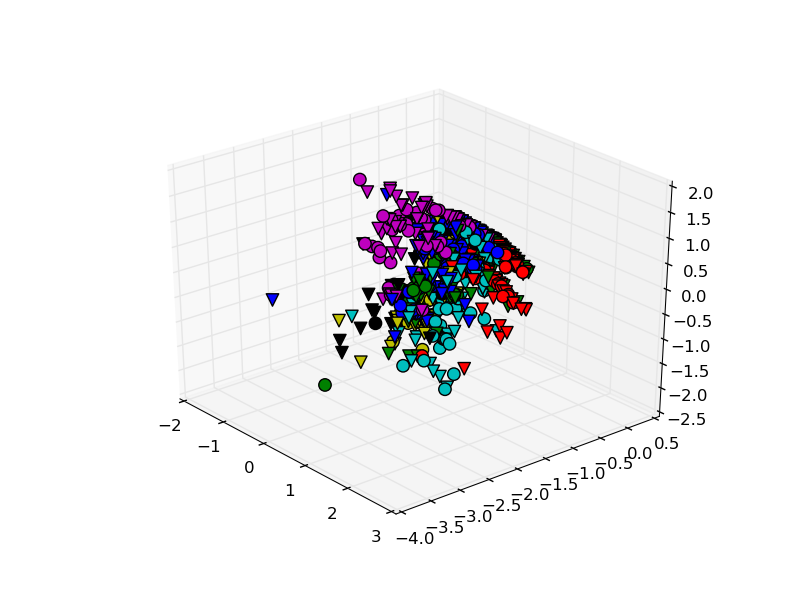
\includegraphics[width=0.5\textwidth]{img/ej1_oja_01_320}

En este grafico podemos observar donde grupos del mismoe lemento estan separados, como por ejemplo el violeta. Tambien observamos puntos outliers, dejando evidencia de que no llegaron a agruparse. 

En general se nota que las distintas categorias se mezclan intensamente y en casi ningun lado se llega a apreciar una categoria bien formada.

En algunas vistas (por ejemplo la ante ultima) vemos que no estan comprimidos, ni se nota una correlacion entre colores.

Como en la experimentacion anterior, se nota que tien mas problemas con el verde y el amarrillo que con el resto.


Por otro lado, analizando todos los graficos de las soluciones obtenidas deducimos que una mejora solucion (decision tomada analizando visualmente los graficos) es la siguiente:

Con un epsilon de 0.05 en sanger obtuvimos un grafico como el siguiente:


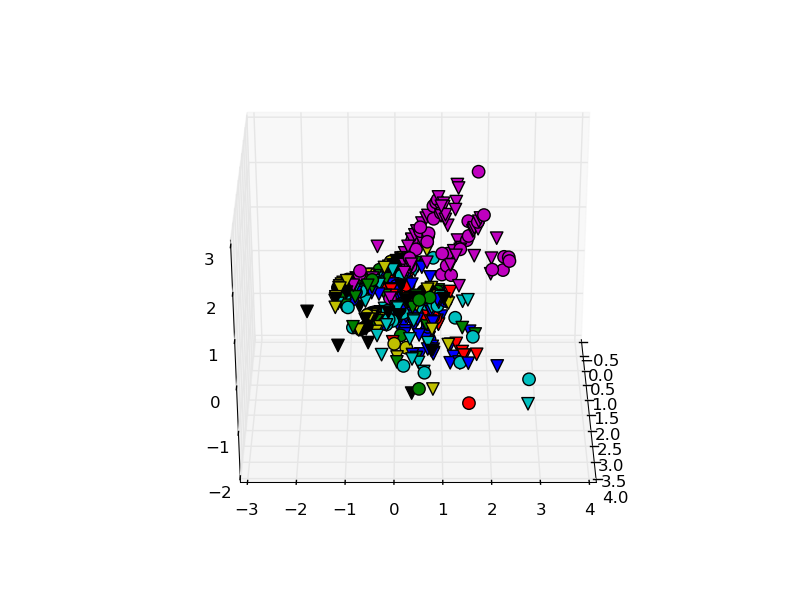
\includegraphics[width=0.5\textwidth]{img/ej1_sanger_005_20}
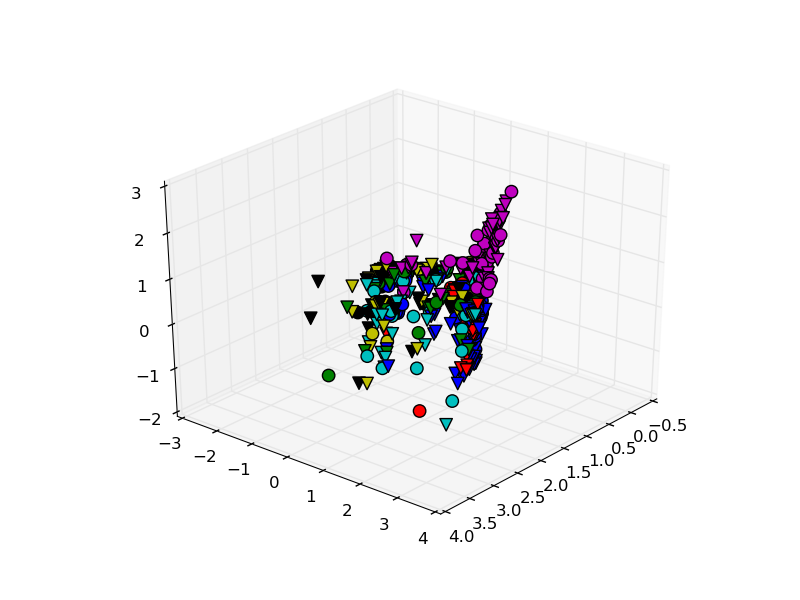
\includegraphics[width=0.5\textwidth]{img/ej1_sanger_005_40}
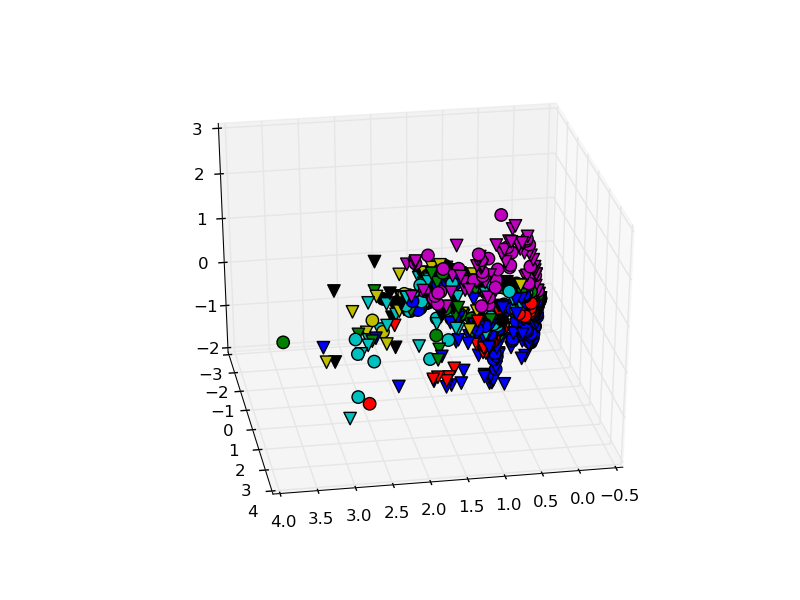
\includegraphics[width=0.5\textwidth]{img/ej1_sanger_005_80}
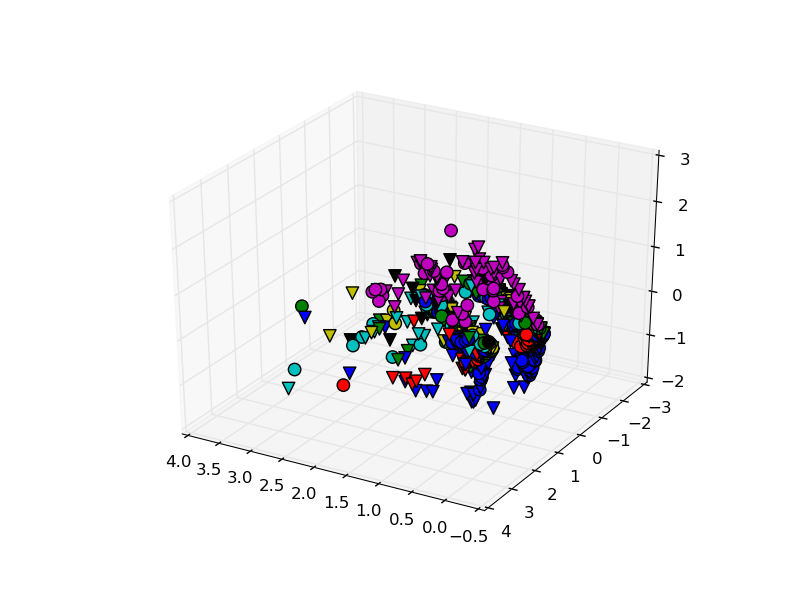
\includegraphics[width=0.5\textwidth]{img/ej1_sanger_005_120}
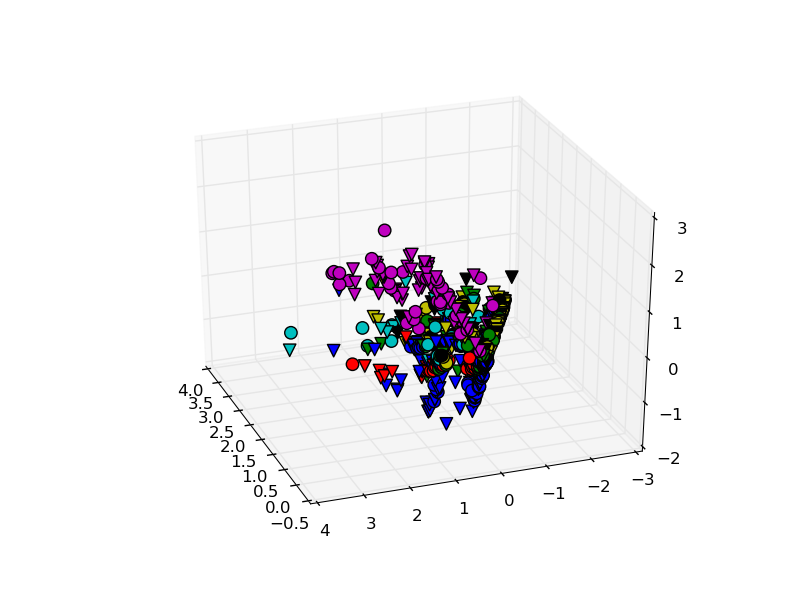
\includegraphics[width=0.5\textwidth]{img/ej1_sanger_005_160}
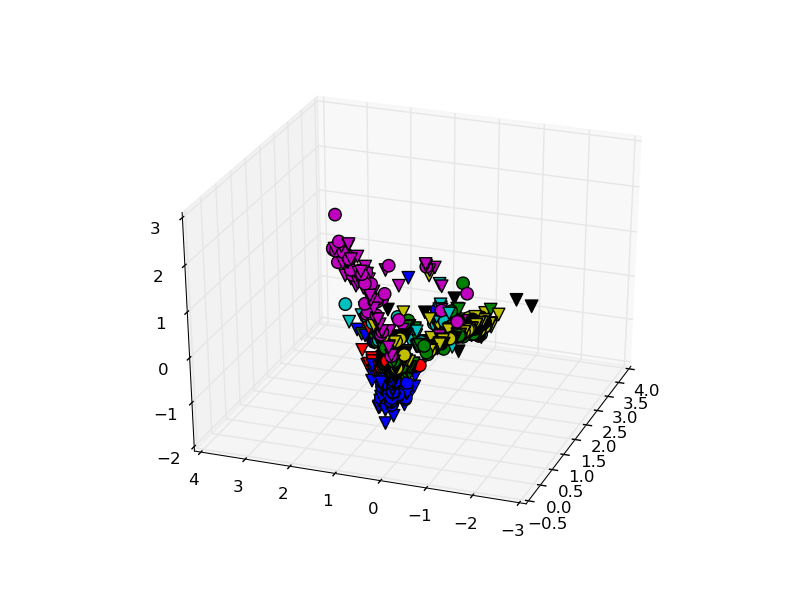
\includegraphics[width=0.5\textwidth]{img/ej1_sanger_005_200}


En estos graficos notamos claramente que el color violeta se separa en una categoria bien definida. 

Por otro lado, en estos graficos, a diferencia de los anteriores, se puede notar como el color azul tambien esta definiendo mejor la discretizacion que en experimentos anteriores.

En el ultimo grafico podems notar claramente la semaparacion entre el violeta y el azul, pero de igual manera vemos que el verde y amarrillo siguen mezclados, por suerte, no tanto como antes, pero siguen mezclando.

Con un epsilon de 0.05 y un Learning Rate de 0.001 en Oja obtuvimos:

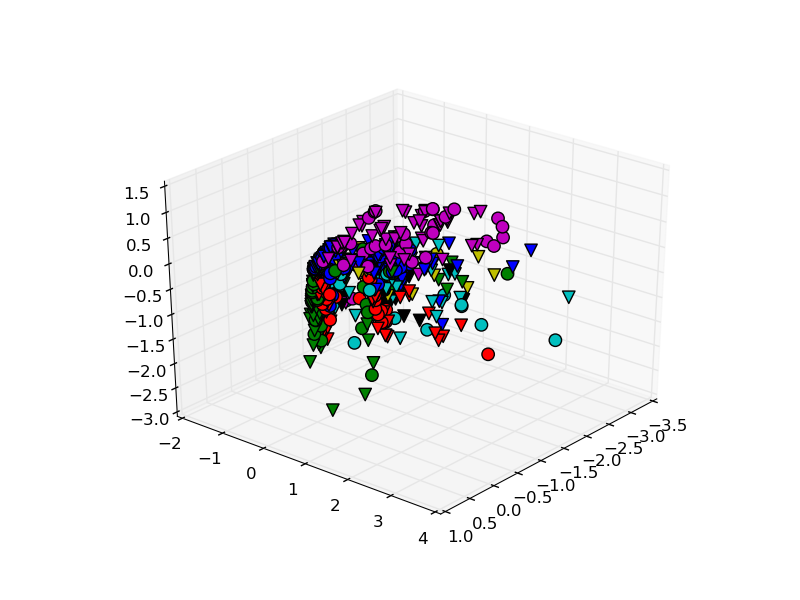
\includegraphics[width=0.5\textwidth]{img/ej1_oja_005_20}
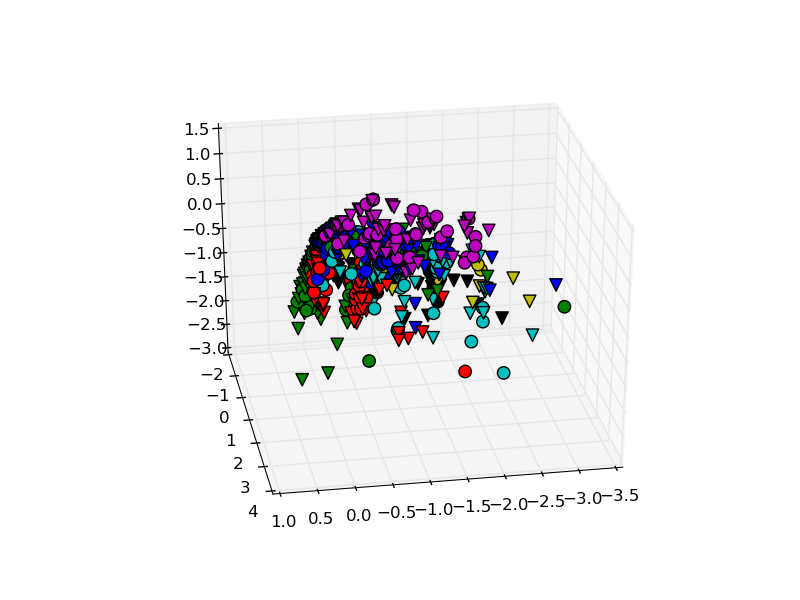
\includegraphics[width=0.5\textwidth]{img/ej1_oja_005_80}
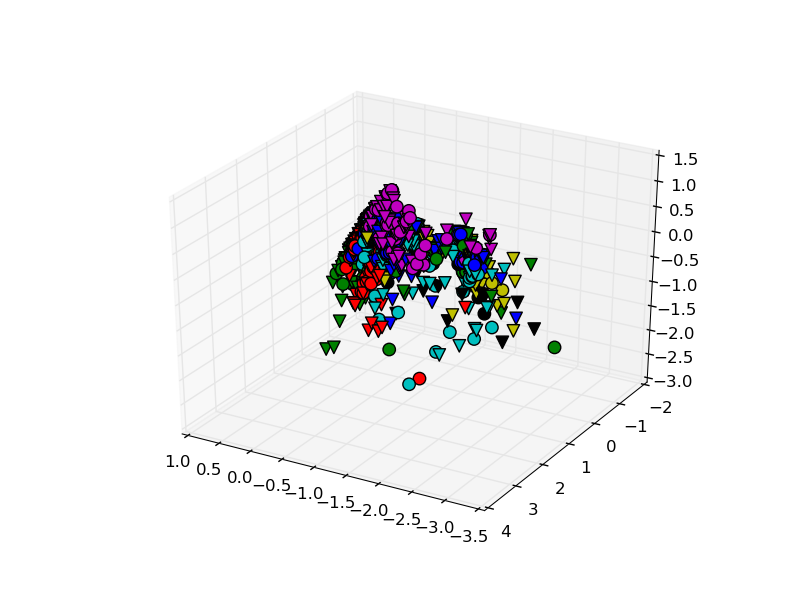
\includegraphics[width=0.5\textwidth]{img/ej1_oja_005_120}
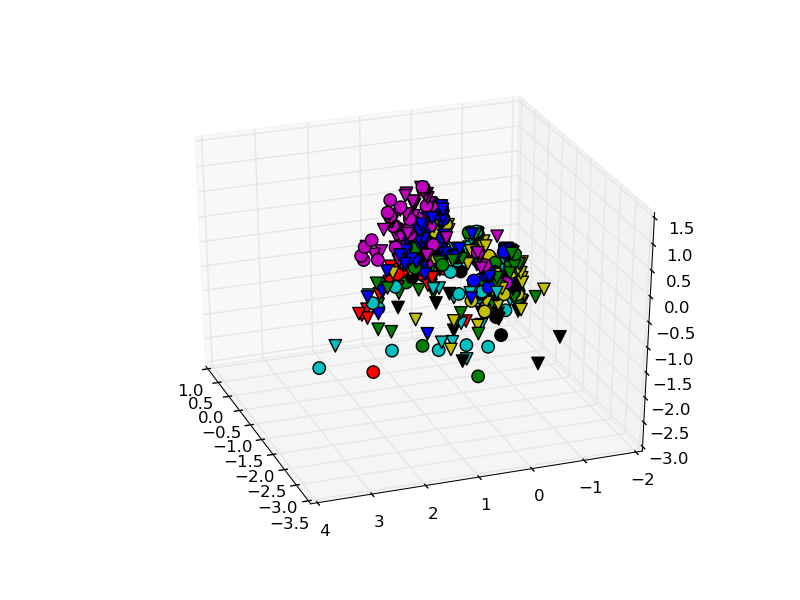
\includegraphics[width=0.5\textwidth]{img/ej1_oja_005_160}
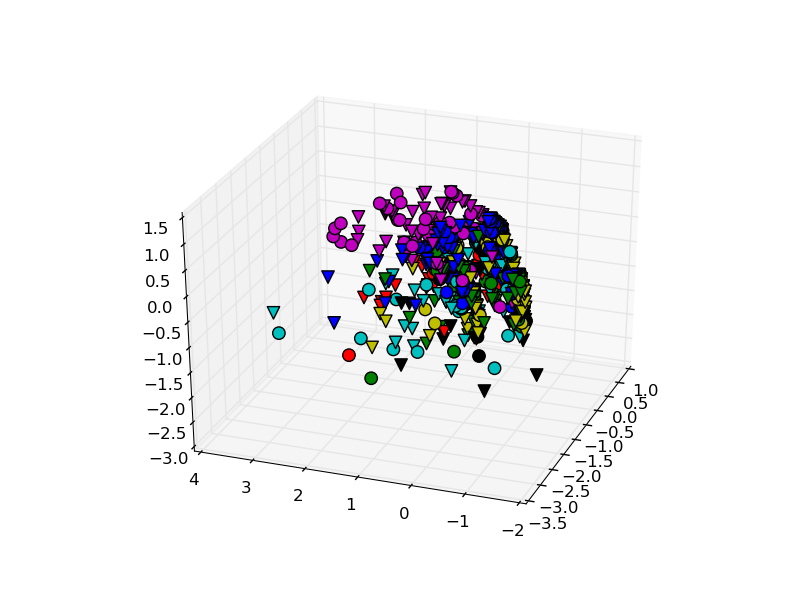
\includegraphics[width=0.5\textwidth]{img/ej1_oja_005_200}
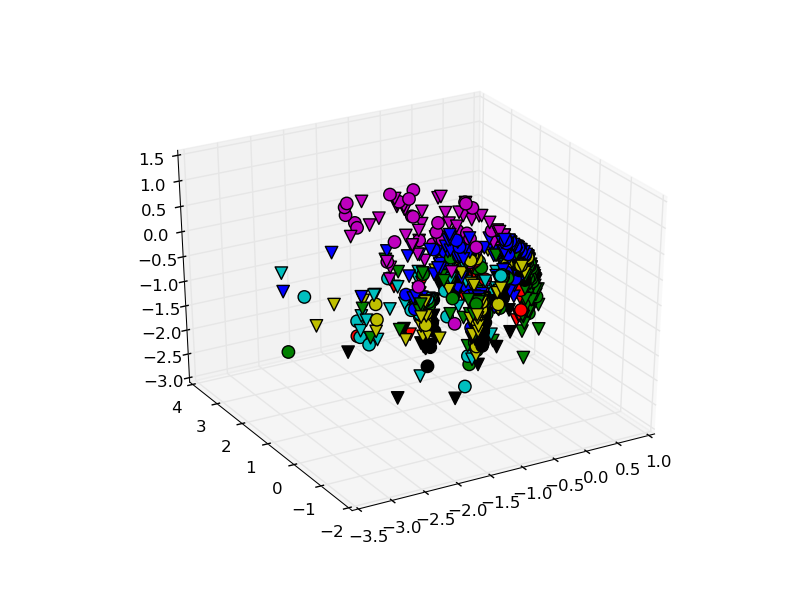
\includegraphics[width=0.5\textwidth]{img/ej1_oja_005_240}

En este grafico vemos, como en el anterior que el color violeta se agrupa de forma correcta.

Del mismo modo que el color azul. Lo mas notable de este grafico es que el color rojo empieza a aparecer en una especie de \textbf{categorizacion}, detalle que antes no pasaba. 

Otro factor importante es que el color verde y el amarillo no se mezclan tanto como en graficos anteriores.

\subsubsection{Conclusion}

Luego de analizar los graficos y resultados del ejercicio 1, podemos concluir que al contrario de lo que esperabamos, en lugar de agruparse en distintas esferas bien definidas, los resultados dieron mas heterogeneos.

Concluimos que la mejor solucion es la ultima proporcionada por Oja (epsilon: 0.05 y learning rate: 0.001), debido a las justificaciones explicadas previamente. En general, se observa que las categorias estan mejor agrupadas.

En general, notamos que los gr\'aficos poseen unas lineas de colores bien definidas, esto es, asumiendo que las categorias son ortoganles, porque cada categor\'ia trata de ajustarce a una dimension, y al haber 9 categorias no alcanzan lsa dimenseiones, por lo tanto vemos estos solapamientos.

\subsection{Ejercicio 2}

Para el ejercicio 2, implementamos un algoritmo para probar distintas dimensiones (cuadradas) de espacio de salida e ir variando los \textbf{Sigma} y \textbf{Epocas}, para ver como influyen, en manera general, en la agrupacion. Para ello, cada una de las corridas se guardan los graficos resultantes y se analiza su comportamiento.

Una vez conseguidos todos los graficos hicimos un analisis observando cual tiene una mejor agrupacion, al igual que en el ejercicio 1, pero esta vez en el plano.


\begin{lstlisting}[caption=pruebas]
	
def prueba():
	file="tp2_training_dataset.csv"
	train_data = np.genfromtxt(file, delimiter=',',usecols=range(1,857))
	train_data=train_data[:600]
	test_data  = np.genfromtxt(file, delimiter=',',usecols=range(0,857))
	if not os.path.exists("imgs/ej2"):
		os.makedirs("imgs/ej2")
	for epoca in [5,10,25,100,500,1000,1500]:
		for M in [3,5,9,20,30,40]:
			for sigma in np.linspace(0.001, 1, 20):
				img_name="imgs/ej2/train_M_"+str(M)+"_sigma_"+str(sigma)+"_epocas_"+str(epoca)+".png"
				print img_name
				red = som(M, M,sigma)
				red.train(train_data,epoca)
				graficador(red,test_data[:600],img_name)
				img_name="imgs/ej2/test_M_"+str(M)+"_sigma_"+str(sigma)+"_epocas_"+str(epoca)+".png"
				graficador(red,test_data[600:],img_name)

\end{lstlisting}

Como se explic\'o anteriormente se corri\'o nuestro algoritmo de pruebas para encontrar las mejores soluciones. El algoritmo de pruebas corrio con estos \textbf{M1} y \textbf{M2}:

\begin{tabular}{|l|l|}
\hline
M1 & M2 \\ \hline
3 & 3 \\ \hline
5 & 5 \\ \hline
9 & 9 \\ \hline
20 & 20 \\ \hline
30 & 30 \\ \hline
40 & 40 \\ \hline
\end{tabular}

y estas epocas
\begin{tabular}{|l|}
\hline
Epocas\\ \hline
100 \\ \hline
500 \\ \hline
1000 \\ \hline
1500 \\ \hline
\end{tabular}

Los resultados de el entrenamiento(izquieda) vs test (derecha) comparando diferentes dimensiones y una epoca de 500. Dado que fueron resultados similares, se exponen los m\'as representativos.

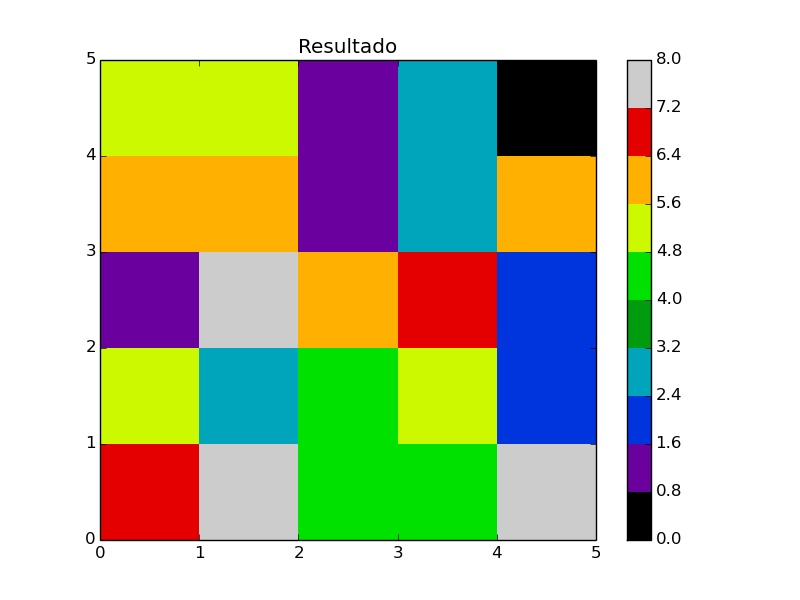
\includegraphics[width=0.5\textwidth]{img/ej2_train_M_5_lrate_001_epocas_500}
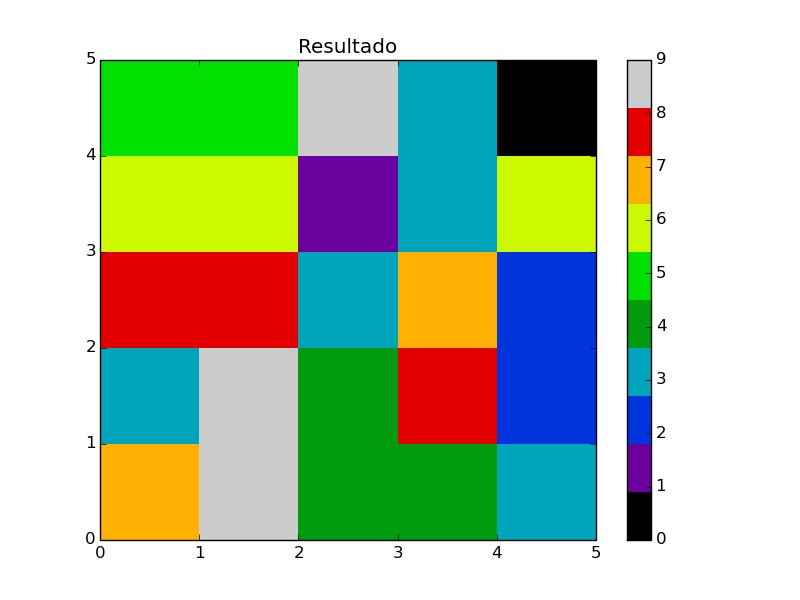
\includegraphics[width=0.5\textwidth]{img/ej2_test_M_5_lrate_001_epocas_500}
{\footnotesize Entrenamiento vs Testing Red 5x5 Learning Rate 0.001 Epocas 500\par}

Como se puede observar a simple vista, la clasificacion obtenida por el test no es consistente con la obtenida en el entrenamiento. Esto puede deberse a que la reduccion de 900 dimensiones a solo 5x5 comprime demasiado la informacion y no es suficiente para agruparlas. Este mismo efecto se observo en las redes de 3x3.

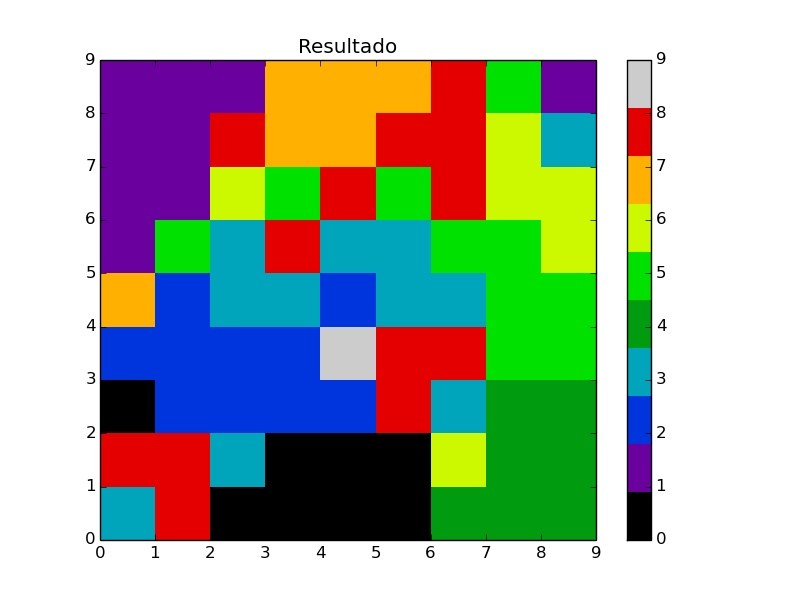
\includegraphics[width=0.5\textwidth]{img/ej2_train_M_9_lrate_001_epocas_500}
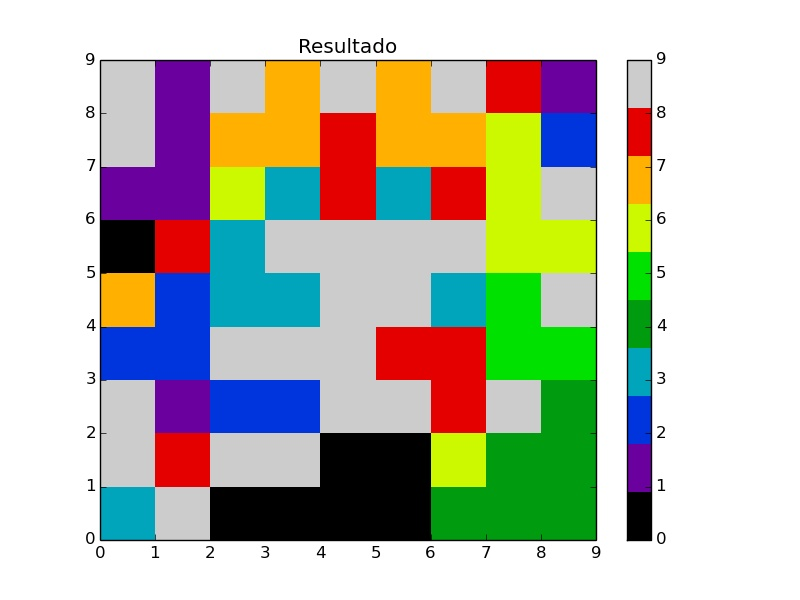
\includegraphics[width=0.5\textwidth]{img/ej2_test_M_9_lrate_001_epocas_500}
{\footnotesize Entrenamiento vs Testing Red 9x9 Learning Rate 0.001 Epocas 500\par}

A diferencia del anterior, se empiezan a notar grupos bien definidos, a excepcion del rojo. Este grupo debe compartir caracteristicas de los otros ocho y por este motivos se deben estar mezclando. 

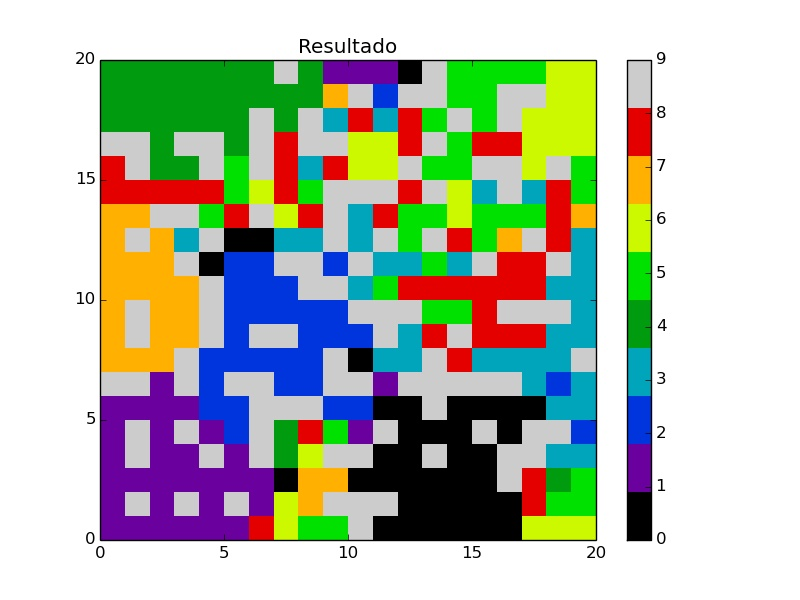
\includegraphics[width=0.5\textwidth]{img/ej2_train_M_20_lrate_001_epocas_500}
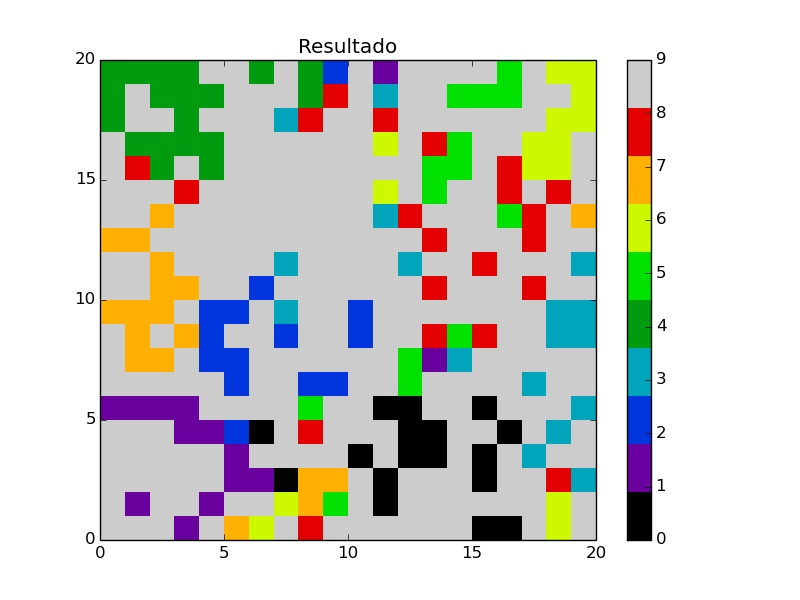
\includegraphics[width=0.5\textwidth]{img/ej2_test_M_20_lrate_001_epocas_500}
{\center \footnotesize Entrenamiento vs Testing Red 20x20 Learning Rate 0.001 Epocas 500\par}

Como se esperaba, al incrementar el espacio de salida y reducir la compresion, los colores se separan m\'as y se agrupan mejor. Se nota una mejora sobre el rojo pero los grupos de color aun presentan puntos de color diferentes.

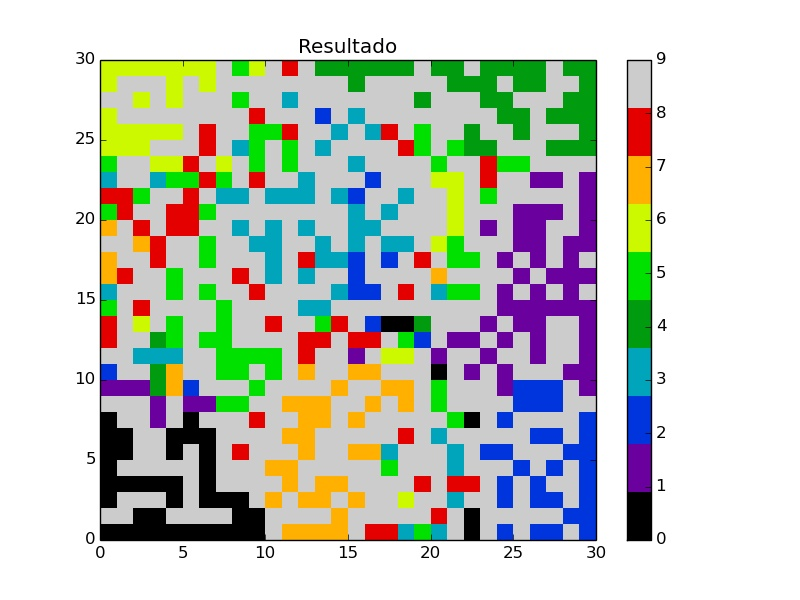
\includegraphics[width=0.5\textwidth]{img/ej2_train_M_30_lrate_001_epocas_500}
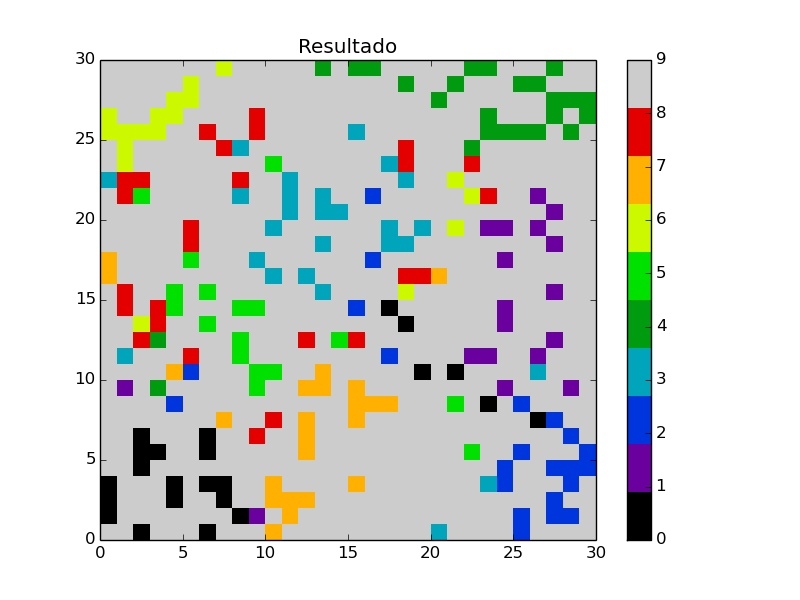
\includegraphics[width=0.5\textwidth]{img/ej2_test_M_30_lrate_001_epocas_500}
{\footnotesize Entrenamiento vs Testing Red 30x30 Learning Rate 0.001 Epocas 500\par}

En este espacio, donde cada punto tiene su equivalente con el espacio de entrada, se aprecia la misma tendencia de grupos que en el caso anterior de 20x20. Pero a su vez, se notan una gran cantidad de neuronas sin activar, sobre todo en la fronteras de los grupos verde oscuro, violeta, azul y negro. El grupo naranja queda definido en la zona central inferior y bastante aislado del resto. Adem\'as, notamos que el color rojo establece un cord\'on alrededor del color verde claro y el turquesa, por lo que esta clasificaci\'on es una categoria que implicar\'ia varias disciplinas. Suponemos que esta es la raz\'on por la cual redes de menor tama\~no no pudieron agrupar bien el color rojo.

Un patron notable en todas las pruebas es que los grupos nunca aparecen en la misma posici\'on, incluso con los mismos par\'ametros. Esto puede deberse a la aleatoriedad para inicializarlos

Ahora compararemos los resultados de el entrenamiento(izquierda) vs test (derecha) en base al tiempo de entrenamiento. Si bien se experimento con todas las dimensiones, dado que los mejores resultados para el caso anterior se obtuvieron con dimension 20x20 y 30x30 solo se mostrar\'an los resultados obtenidos por estas instancias.


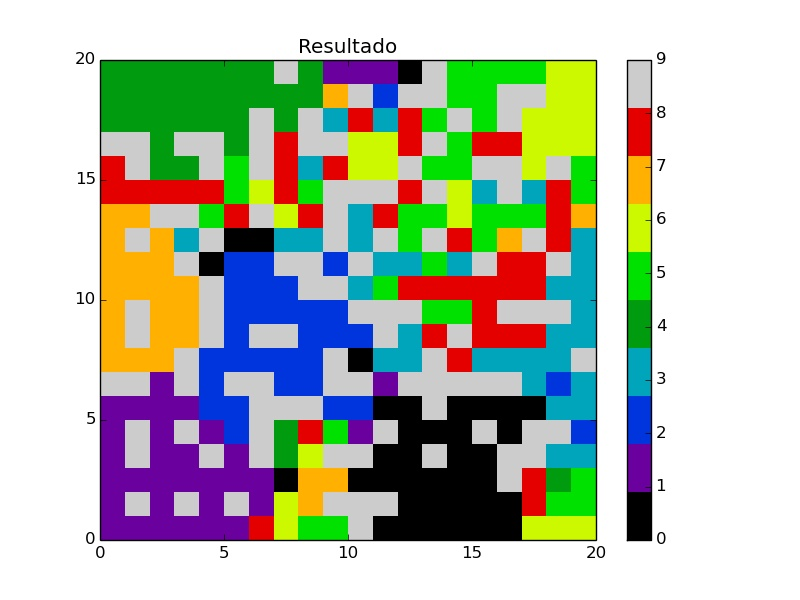
\includegraphics[width=0.5\textwidth]{img/ej2_train_M_20_lrate_001_epocas_500}
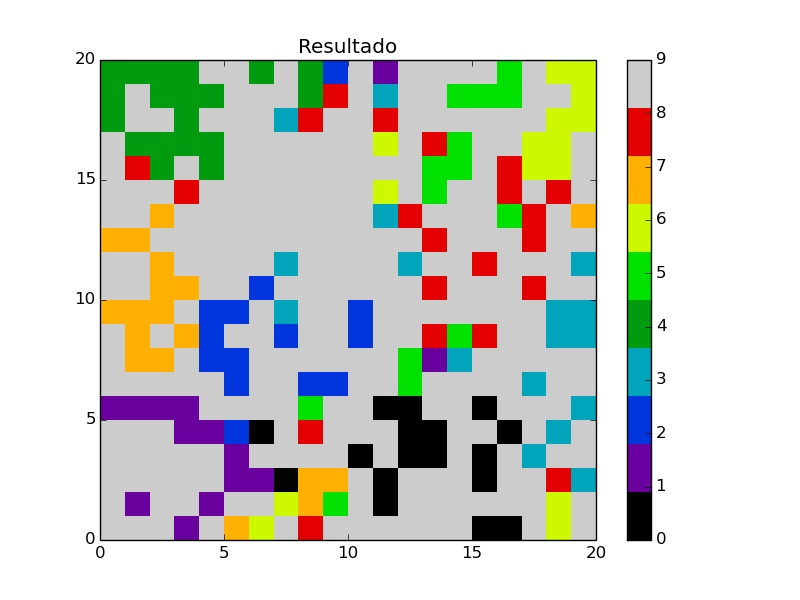
\includegraphics[width=0.5\textwidth]{img/ej2_test_M_20_lrate_001_epocas_500}
{\center \footnotesize Entrenamiento vs Testing Red 20x20 Learning Rate 0.001 Epocas 100\par}
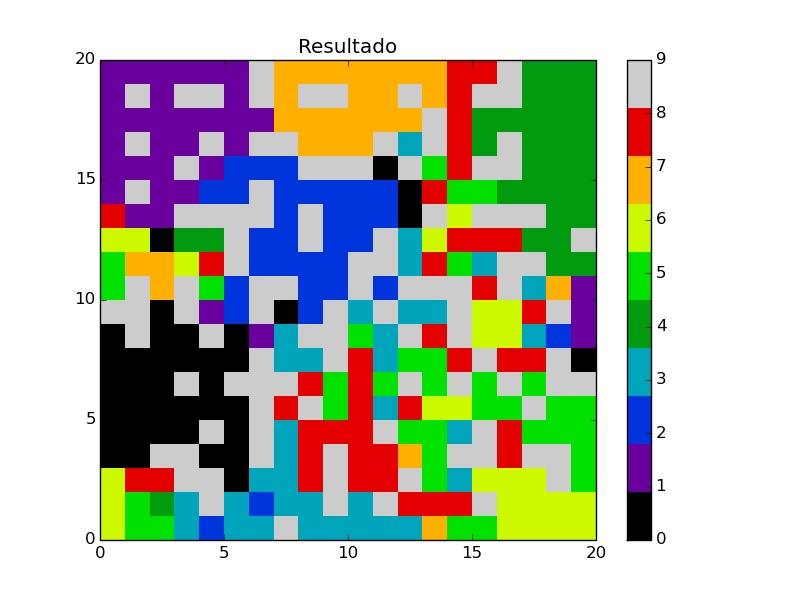
\includegraphics[width=0.5\textwidth]{img/ej2_train_M_20_lrate_001_epocas_1000}
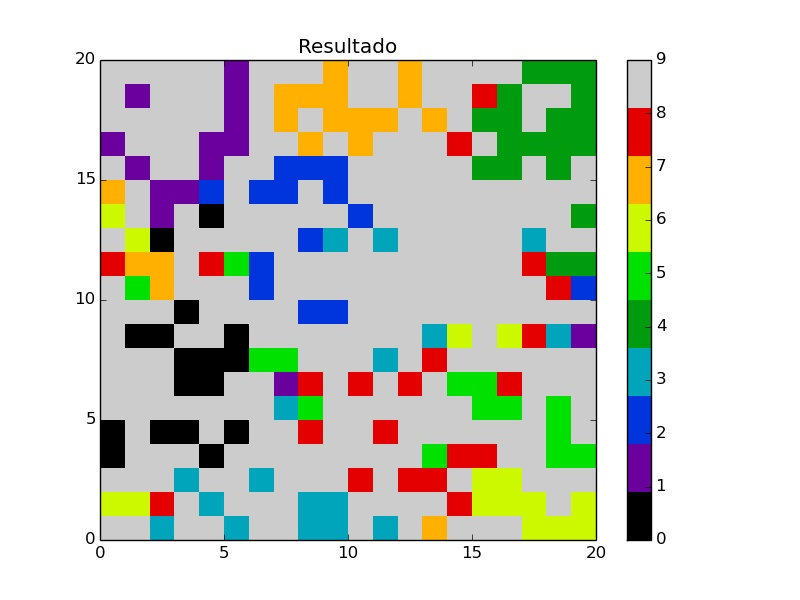
\includegraphics[width=0.5\textwidth]{img/ej2_test_M_20_lrate_001_epocas_1000}
{\center \footnotesize Entrenamiento vs Testing Red 20x20 Learning Rate 0.001 Epocas 500\par}
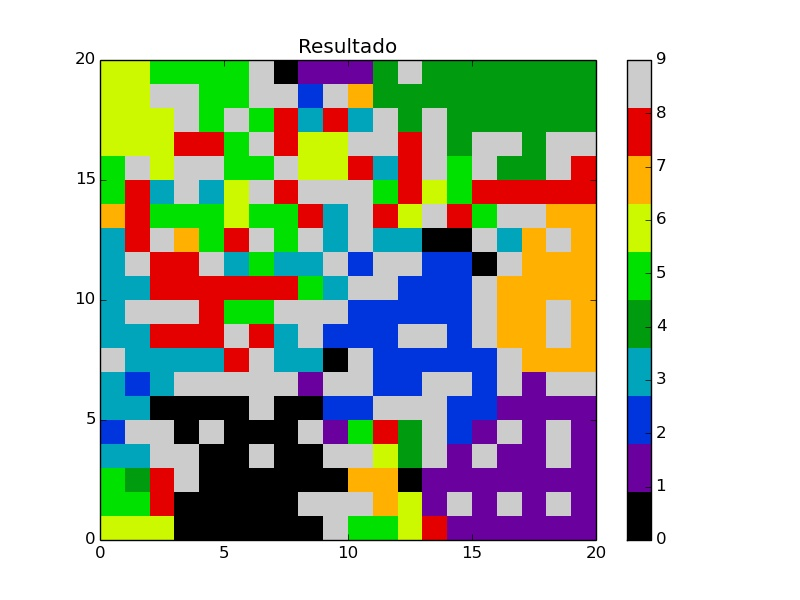
\includegraphics[width=0.5\textwidth]{img/ej2_train_M_20_lrate_001_epocas_1500}
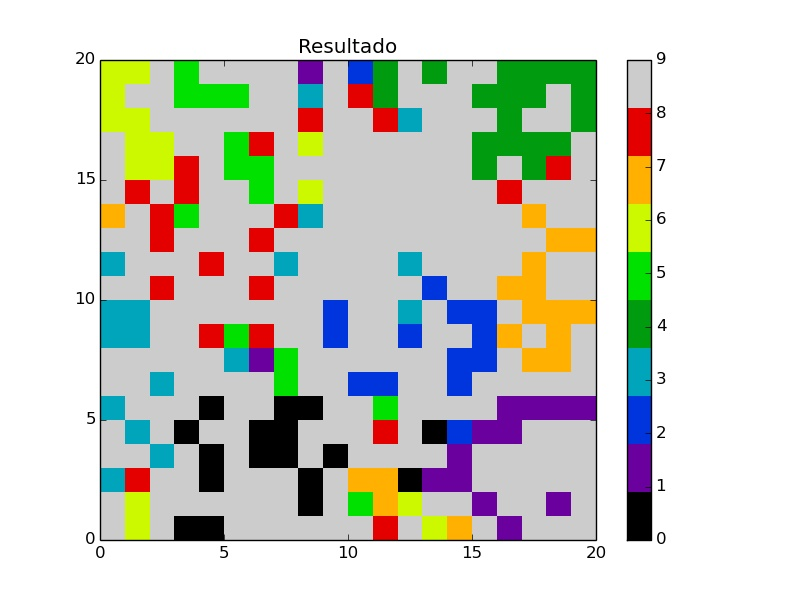
\includegraphics[width=0.5\textwidth]{img/ej2_test_M_20_lrate_001_epocas_1500}
{\center \footnotesize Entrenamiento vs Testing Red 20x20 Learning Rate 0.001 Epocas 1000\par}

Curiosamente, no existe una mejora en la solucion para epocas mayores a 100 para cualquier learning rate entre 0.1 y 0.001.

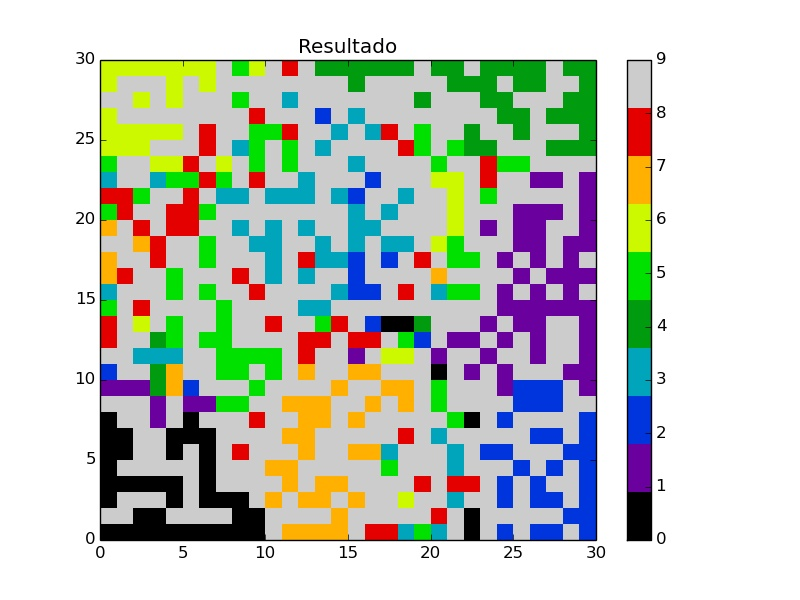
\includegraphics[width=0.5\textwidth]{img/ej2_train_M_30_lrate_001_epocas_500}
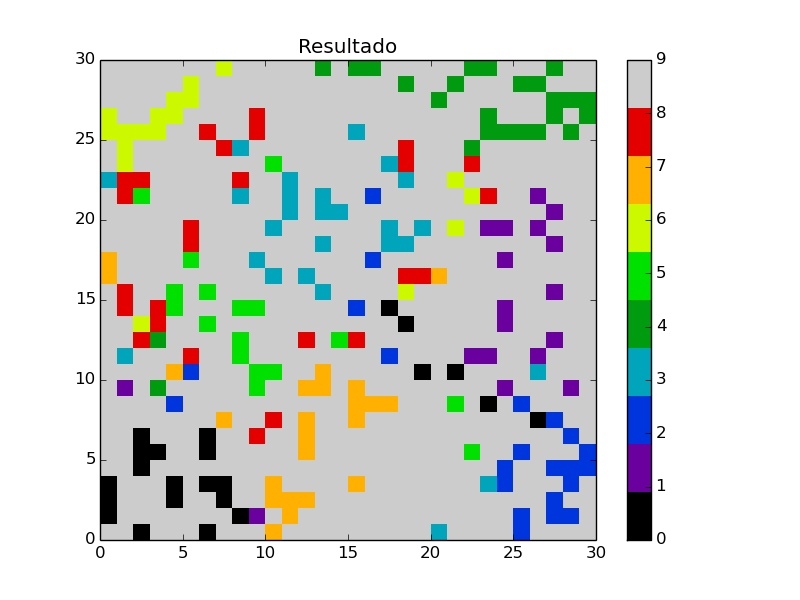
\includegraphics[width=0.5\textwidth]{img/ej2_test_M_30_lrate_001_epocas_500}
{\footnotesize Entrenamiento vs Testing Red 30x30 Learning Rate 0.001 Epocas 100\par}
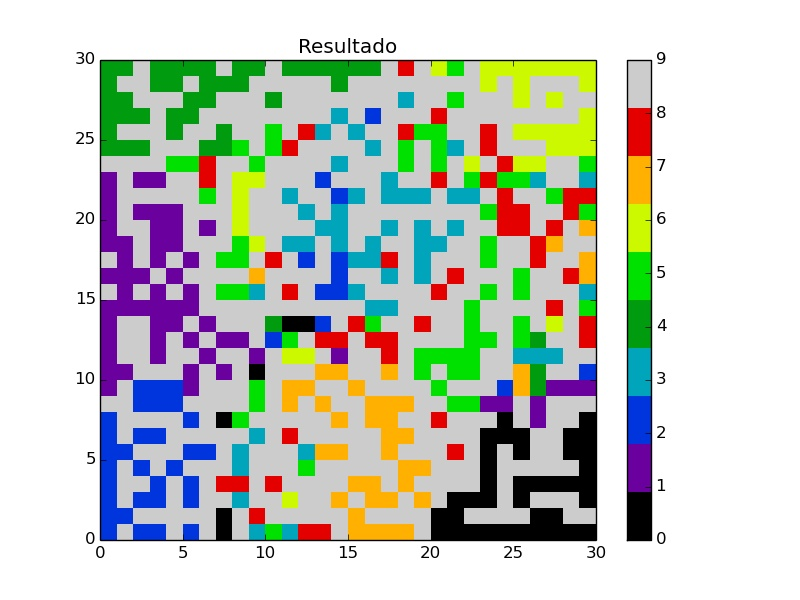
\includegraphics[width=0.5\textwidth]{img/ej2_train_M_30_lrate_001_epocas_1000}
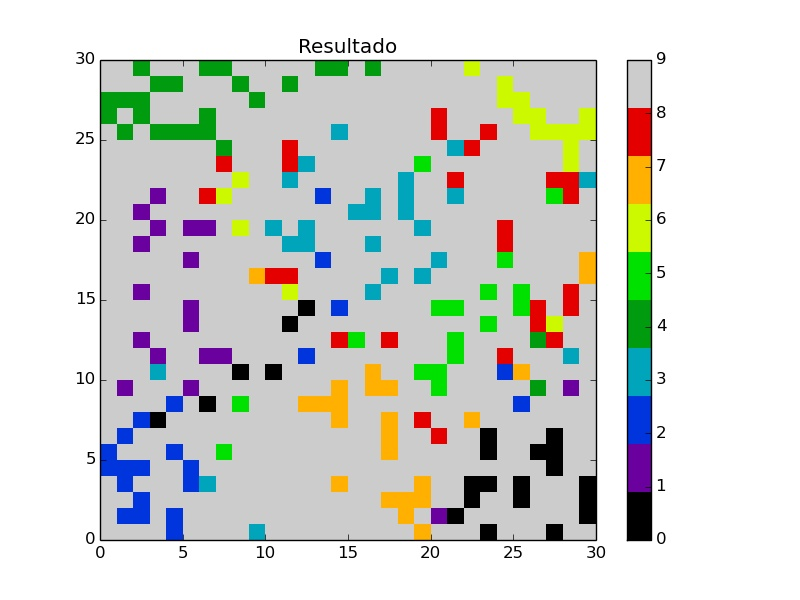
\includegraphics[width=0.5\textwidth]{img/ej2_test_M_30_lrate_001_epocas_1000}
{\footnotesize Entrenamiento vs Testing Red 30x30 Learning Rate 0.001 Epocas 500\par}
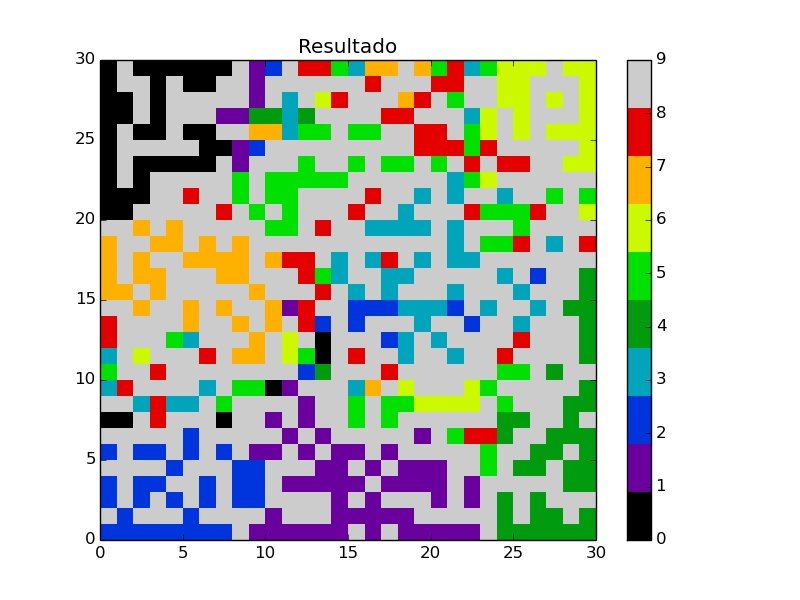
\includegraphics[width=0.5\textwidth]{img/ej2_train_M_30_lrate_001_epocas_1500}
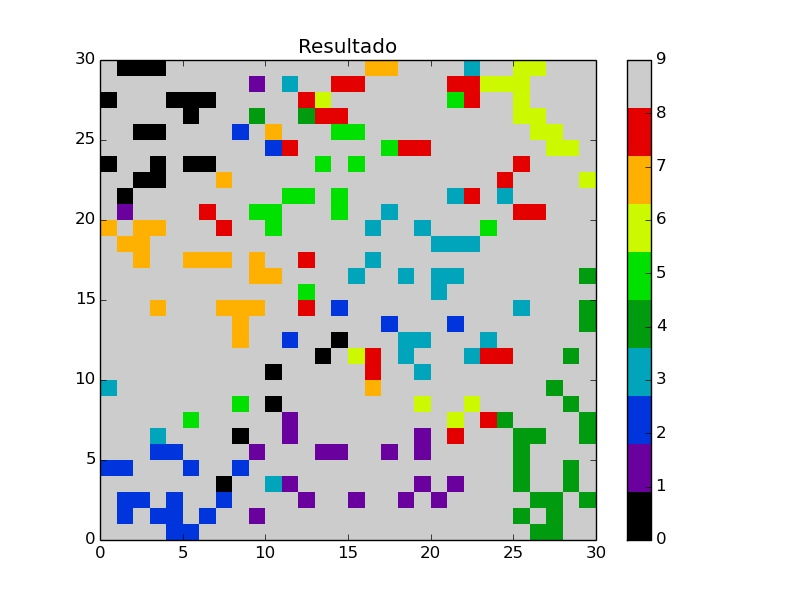
\includegraphics[width=0.5\textwidth]{img/ej2_test_M_30_lrate_001_epocas_1500}
{\footnotesize Entrenamiento vs Testing Red 30x30 Learning Rate 0.001 Epocas 1000\par}

Si bien no hay una mejora en calidad de soluci\'on, es necesario aclarar que aunque terminen en la misma cantidad de epocas, el tiempo de computo de la solucion de la red de 30x30 es mucho mayor que la de 20x20. Por este motivo, la corrida de la red de 40x40 no se pudo realizar para mediciones mayores a 500 epocas.

\subsubsection{Conclusion}

Luego de analizar los graficos y resultados del ejercicio 2, podemos concluir que las dimensiones de la red no solo influyen en la calidad de la solucion sino tambien en el tiempo de calculo de la misma. 

En base a todo lo anterior, decidimos que la mejor solucion es una red de 30x30 con un learning rate de 0.01 y 100 epocas de entrenamiento. Esta red provee una buena clasificacion y balancea el costo en tiempo.

Esperabamos que el learning rate alterara significativamente el mapeo. Sin embargo, al utilizar la funcion sigma
eta = t ** (- 1/2) y sigma = (M2/2)* (t ** (-1/3)), creemos que acorto mucho el campo de vecinos que modifica la unidad ganadora, por lo cual, el cambio producido fue poco.

